\chapter{Independent compositions of \mw{Brut y Brenhinedd}}
\label{cha:indep-comp-mwbr}
This chapter analyses the orthography of lenition in the Welsh translations of the  \lat{Historia Regum Brittanniae} by Geoffrey of Monmouth, a Latin-language historical prose text dating from the twelfth century.
Translations of this text into Welsh date from the thirteenth century onwards.
In total, there are some sixty manuscripts containing some sort of translation or rendition of this history, and they may be divided into six individual classes.
Each of these classes contains independent translations of the Latin text; some of them may be considered faithful translations, whereas others handle the source material more freely~\autocite[xxiv-xxxi]{roberts_brut_1971}.

The existence of several independent translations or reworkings of a single text made over much of the \gls{mw} period is valuable in studying linguistic or orthographical developments.
These texts are valuable because their manuscript witnesses are roughly contemporaneous with the composition of their translation.
Additionally, the independence of these translations means that each version makes for a reliable snapshot of the language and orthography of its time and place.
At the same time, the fact that all the \gls{mw} texts are translations of the same text in Latin offers a controlled research environment:  any difference in the language of the translations cannot be due to differing subject matter.
As such, differences in the Welsh translations are controlled for the variable of subject matter.
The importance of comparing texts containing similar lexical content is shown by \textcite{Wil_Lexical05}, who shows that language change in \gls{mw} may occur at different times for different words.
Comparing different translations of the same text ensures that a lexical item occurring frequently in one translation should occur similarly frequently in another.
Similarly, we know that the translations of are all translations from Latin, meaning the variable of source language is also controlled for.
Geoffrey of Monmouth's Latin is generally straightforward, and his vocabulary and grammar do not generally give any trouble~\autocite[lxxvi]{Geo_History09}.
The independence of these translations and the concurring independence of orthographies contrasts with the law texts discussed in Chapter~\ref{cha:welsh-laws}, as those law texts tend to be Welsh-language copies of Welsh-language texts, carrying over some old orthography.
The fact that we deal with translations of a Latin text means that any occasions where lenition may give rise to ambiguities may be resolved by comparing the Welsh to the Latin.
However, medieval translations are not necessarily faithful to the original:
\tqt{\begin{welsh}
  Nid yw'r cyfieithwyr hyn, fwy na chyfieithwyr cyffredin y cyfnod canol, yn gaeth i'r testun Lladin. [\dots] Newidir rhai manylion neu ychwanegu rhai brawddegau er mwyn cysylltu'r hanes â ffynonellau eraill.%
\end{welsh}%
\footnote{These translators are not slavish to the Latin text any more than typical translators of the medieval  period. [\dots]
  Some details are changed, or some sentences are added in order to connect the history with other sources.}}{Rob_Testunau74}{290}
Nevertheless, the subject matter of each text --- no matter how many details are altered --- remains historiography, so wildly differing rates of lenition found in each translation cannot possibly be caused by differing subject matter found in each manuscript.

Caution is needed when dealing with translations if the language of the original Latin seeps through into the grammar of the Welsh.
The result of this is that some constructions are more frequent than would be expected in a Welsh prose text:
\tqt{
  \begin{welsh}
    Gadawodd y Lladin ei hôl ar arddull y cyfieithiadau, yn yr ansoddeiriau lluosog, a'u safle o
flaen yr enw, yng nghytundeb berf â'i goddrych, yn y gystrawen berthynol, yn y defnydd o enwau
haniaethol, ac o ansoddeiriau berfol i gyfleu rhangymeriad gorffennol, yn y trosi llythrennol o
elfennau gair cyfansawdd, yn y cystrawennau trwsgl a'r colli gafael ar rediad brawddeg wrth geisio
llunio brawddegau cymhleth yn hytrach na brawddegau cydradd, byrion y testunau brodorol.%
  \end{welsh}%
\footnote{The Latin left its mark on the form of the translations, in the plural adjectives, and their place before the noun, in the agreement of the verb with its subject, in the relative clause, in the use of abstract nouns, and of verbal adjectives to convey past participles, in literally translating elements of compound words, in the clumsy sentences and in losing the grip on the flow of a sentence from trying to fashion complex sentences instead of the coordinate, short sentences of the original texts.}
}{Rob_Testunau74}{289}
The most important point here is the placement of adjectives before the noun they qualify.
Wherever this happens, the element following the preposed adjective is lenited.
The use of these adjectives is possible in Welsh, but is highly stylized%
\footnote{Adjectives that always come before the noun they modify, \eg \mw[old]{hen}, are not highly stylized in this position.}.
Because translating from Latin brings preposed adjectives out more frequently in Welsh they may have been misunderstood occasionally, as they caused some erratic behaviour, as found in Example~\ref{ex:wychyrcalet}.
There is also a more obvious feature showing these texts were translated from Latin: Latin personal names are found and code switching to Latin also occurs.  

All in all, their syntax shows these translations tend to be slavish on the sentence level compared to present-day translations, but freely deviate from the Latin original in terms of content. 





\section{Versions used}
I have taken four different manuscript witnesses of \mw{Brut y Brenhinedd} from four classes for analysis.
Three of these are thirteenth-century manuscripts, and the fourth is from the fourteenth century.
\Textcite{Rob_Testunau74}  notes that these three translations  are similar in terms of how well they are translated.  
\tqt{
  \begin{welsh}
    Fe'i  cyfieithwyd [yr \textit{Historia}] deirgwaith yn  y drydedd ganrif ar ddeg, ac ymddengys fod dau o'r fersiynau hyn, sef hwnnw sydd yn Peniarth 44, a'r un sydd yn Llansteffan 1, yn perthyn i flynyddoedd cynnar y ganrif.
    Dichon fod y trydydd, fersiwn Brut Dingestow, ychydig yn ddiweddarach.
    Y mae iaith y tri fersiwn yn debyg, a chyffelyb hefyd yw safonau'r cyfieithwyr a'u hagwedd at y testun Lladin.%
  \end{welsh}%
\footnote{The [Historia] was translated three times in the thirteenth century, and it appears that two of these versions, \ie the one that is in Peniarth 44, and the one that is in Llansteffan 1, belong to the early years of the century. It seems that the third, the  Brut Dingestow version, is a bit more recent. The language of the three versions is similar, and the standards of the translators and their attitude towards the Latin texts are also similar.}
}{Rob_Testunau74}{288--289}
\Textcite[xxix]{roberts_brut_1971} notes that all three translations are `close renderings of the Latin', and that all translations are independent.
This makes all of these three  manuscripts good independent snapshots of thirteenth-century orthography.
However, when the methods of translation between these three versions are compared, some differences may be identified \autocite{Rob_Testunau74}.
While the \gls{ll1} translation is the most faithful one of the three in both style and contents, the \gls{p44} translation is faithful tothe Latin on the level of the individual sentence, but leaves out some parts, and the translation found in \gls{bd} is the freest in terms of style as the text is shortened by summarising rather than selecting parts of the original:
\tqt{
    \begin{welsh}
Er mor debyg yw ymateb y tri chyfieithydd i'r Historia, y mae eu dull o gyfieithu'n amrywio. Gŵr
cydwybodol, gofalus oedd cyfieithydd fersiwn Llansteffan 1. Ychydig iawn a hepgorodd o'r testun
Lladin ond ceisiodd ei drosi frawddeg wrth frawddeg, hyd yn oed yn y manylion. Ef, yn sicr, a
luniodd y cyfieithiad mwyaf ffyddlon, er bod ei arddull braidd yn drwsgl. Yr oedd ei
destun Lladin ef hefyd yn wahanol mewn mannau i'r un a ddefnyddiwyd gan y ddau gyfieithydd
arall. Diddordeb cyfieithydd Peniarth 44 oedd rhediad yr hanes ei hun. Y mae ganddo arddull
weddol naturiol, uniongyrchol ac adroddiadol. Gall fywiogi'r hanes ond ei nodwedd gyffredin yw ei
fod yn ei gwtogi fel yr â rhagddo, trwy dorri allan frawddegau ac adrannau cyfain, nes y ceir ganddo,
erbyn y diwedd, grynodeb go chwyrn o'r Lladin. Llwyddodd cyfieithydd Brut Dingestow yntau i
gwtogi'r hanes, ond ceisiodd ef dalfyrru'n fwy deallus, nid trwy dorri adrannau allan, ond trwy
grynhoi wrth gyfieithu, a thrwy aralleirio, gan gadw'r cyfan o'r hanes, a hynny mewn Cymraeg digon
llyfn at ei gilydd, gydag adleisiau o'r arddull draddodiadol.%
\end{welsh}%
\footnote{However similar the response of the three translators is to the Historia, their method of translation varies. The translator of Llansteffan 1 was a conscientious, careful man. He left out very little of the Latin text, and tried to translate it sentence by sentence, even down to the details. He, surely, composed the most faithful translation, although his style is quite awkward. His Latin text was also different  from the one used by the other two translators in some places. The translator of Peniarth 44 was interested in the flow of the history itself. He has a fairly natural, direct, and narrative style. He may enliven the history, but his general trait is to abbreviate what comes before him, by cutting out whole sentences and parts, so that he gives in the end quite a drastic summary of the Latin. The translator of Brut Dingestow managed to abbreviate the history, but he tried to condense in a more intelligent way, not by cutting out sections, but by summarizing while translating, and by rewording, while keeping the whole of the history, and this in  fairly smooth Welsh on the whole, with echoes of the traditional style.}
}{Rob_Testunau74}{292--293}
These differences notwithstanding, considerable Latin influence is found in all three versions.
An example of this may be found in Examples~\ref{ll1llyr}, \ref{p44llyr}, and \ref{bdllyr}, where each translation has \mw[two daughters]{dwy ỽerchet} with a plural noun following the numeral, following Latin rather than Welsh grammar.

One of the earliest manuscripts containing the \mw{Brut} is \gls{ll1}, which
is dated mid-thirteenth century\todo{ref from Huws}.  A part of
the manuscript contains another version, namely a fragment
of \gls{p44}. The scribe was not a translator, as may be judged from
some mistakes and omissions~\autocite[xxxvii]{roberts_brut_1971}. This manuscript is shown by \textcite[80--81]{Rod_Datable98} to have comparatively high incidence of preterite ending \mw[]{-awdd} compared to \mw[]{-wys} for its period. 
I used lenition on pages 33 to 38 for analysis.



The \gls{p44} translation of the \mw{Brut} is roughly as old as the \gls{ll1} one, although \textcite[85]{Rus_Orthography93} argues on orthographic grounds that it is written before \gls{ll1}. The manuscript is written by the same hand as \gls{sC}, discussed in Chapter~\ref{cha:welsh-laws}.
\Textcite[xix]{Lew_Brut42} states that \gls{p44} and \gls{ll1} are based on a common original translation, undoubtedly because the \gls{ll1} manuscript contains a fragment of the \gls{p44} translation, but according to \textcite[xliii--xliv]{Rob_Astudiaeth69}  they are based on separate translations.
I analysed lenition on pages 23 to 28.

\Gls{bd} is found in the following manuscript: \gls{nlw} MS 5266.
It is dated to the end of the thirteenth century~\autocite[xliii]{Rob_Astudiaeth69}.
An edition of this text is prepared by \textcite{Lew_Brut42}.
His introduction does not mention the orthography of lenition.
I analysed lenition found on pages 26 to 36.




\Gls{bcc} is the latest manuscript under consideration.
It contains the only translation from after the thirteenth century among the texts analysed in this chapter.
It dates from the mid-fourteenth century according to~\textcite[xlv]{Rob_Astudiaeth69}, and from the second quarter of the same century according to \textcite[xviii]{Jon_Brenhinedd71}.
\todo{The scribe of this \mw{Brut y Brenhinedd} translation is identified as scribe X89. (relevant?)}
I took lenition on folios 16r to 19v for analysis.

\Textcite{Rob_Testunau74} notes that the \gls{bcc} translation departs from the original in more ways than just summarizing, as it also incorporates other sources of history:
\tqt{
  \begin{welsh}
Cyfieithiad newydd yw Cotton Cleopatra lle y mae'r gwaith o gymathu â ffynonellau
eraill yn llawer mwy amlwg. Y mae'n fyrrach na'r Historia gan fod y cyfieithydd wedi torri'r areithiau
a llawer o'r disgrifiadau o'r brwydrau, ac wedi hepgor llawer o'r manylion. Ond o'r tu arall, y mae
yma lawer o ychwanegu sy'n gwneud y fersiwn hwn yn fwy storïol na'r un arall.%
\end{welsh}%
\footnote{Cotton Cleopatra is a new translation, where the incorporation of other sources is much more obvious. It is shorter than the Historia because the translator cut out the speeches and many of the descriptions of the battles, after removing many of the details. But on the other hand, there are many additions that make this version more storylike than any other one.}
}{Rob_Testunau74}{293}


\section{Method}
\label{sec:method}
From each manuscript, I have collected instances of orthographical
lenition as well as instances of where orthographical lenition would
be expected, but is not found. The sample used comprises roughly the
story of Llŷr and his daughters.  Some 250 data points are taken
from each manuscript.

\Gls{petr}, both the type resulting from grammatical lenition and from clitic reduction have been collected for prepositions
and (historically) nouns, but not for personal pronouns such
as \mw[I]{mi/fi}. The reason why these forms are included --- albeit
as research exceptions --- is that their orthography also changed over the
thirteenth century\footnote{See \ref{sec:petrification}.}. Including them allows
us to gauge when this happened relatively to \gls{morphophonlen}.
Including them also allows us to understand how easy it is to miss how \gls{morphophonlen} of voiceless stops was barely ever represented in the earliest translations, because \gls{petr} was already common in the same period.

It is not always clear what types of lenition applied in different
stages of \gls{mw}. Particularly some types of \gls{freelen},
such as object lenition and \gls{np} lenition tend to be used only irregularly,
or only in later texts~\autocite{van_development14}, but
with no distinction for consonant type. Evidence for the existence of
lenition differs between texts here, precluding a catch-all policy for
the inclusion of such instances. I generally look for multiple positive
instances attesting to the lenition of objects and \gls{np}s.
Consequently, I do not consider non-lenition of \mw[dead]{marỽ} in
Example~\ref{ex:bvmarw} to be relevant for the orthography of lenition,
because \gls{np} lenition is only found once elsewhere in this corpus.
As it happens, it is found in the same sentence.
This implies that \gls{np} lenition was grammatically optional.
\mwcc[ex:bvmarw]{\gls{ll1} 38.9--10}
{en e tryded wlwydyn gwedy henny e \al{bỽ ỽarỽ} llyr.\ ac e \al{bỽ marỽ} aganyppỽs brenyn ffreync}{In the third year after that Llŷr \al{died}, and Aganippus, king of France, \al{died}.}


\section{An overview of the results}
\label{sec:comparison-versions}
Let us look at one sentence found in all the manuscripts in a similar form.
This sentence demonstrates how the orthography of lenition developed in the thirteenth and fourteenth centuries.
\begin{mwl}
  \mwc[ll1llyr]{\acrshort{ll1} 34.16--18}{Ac ena hep ỽn gohyr
    o \al{k}yghor y \al{w}yrda ef ar rodes e dwy \al{ỽ}erchet hynaf
    ydaỽ yr deỽ \al{t}ewyssaỽc. nyt amgen tewyssaỽc kernyw ac ỽn
    gogled}{And then without any delay of counsel of his noblemen, he
    gave his two eldest daughters to the two princes, none other than the
    prince of Cornwall and the one of [the] North.}
  \mwc[p44llyr]{\acrshort{p44} 24.21--23}{Ac ena ny \al{b}ỽ ỽn gohyr
    o \al{k}yghor y \al{w}yrda er rodes ef e dwy \al{ỽ}erchet hynaf y
    deỽ \al{t}ewyssaỽc nyt amgen a thewyssaỽc kernyw. a thewyssaỽc e
    gogled.}{And then there was no delay of counsel of his noblemen
    that he gave his two eldest daughters to two princes, none other than
    the prince of Cornwall and the prince of the North.}
  \mwc[bdllyr]{\acrshort{bd} 31.6--7}{A hep \al{o}hir
    o \al{g}yt\al{g}yghor y \al{w}yrda y rodes ef y dỽy \al{u}erched
    hynhaf ydaỽ y \al{t}ywyssogyon yr alban.\ a chernyỽ. }{And without
    delay of counsel of his noblemen, he gave his two eldest daughters
    to the princes of Scotland and Cornwall.}
  \mwc[bccllyr]{\acrshort{bcc} 17r.21--24}{Ac yna yn diohir y rodes ef
    y dwy \al{v}erchet hynaf y deu \al{d}ywyssawc nyt amgen tywyssawc
    kernyw ar hwnn yr alban}{And then without delay he gave his two
    eldest daughters to two princes, none other than the prince of
    Cornwall and the one of Scotland.}
\end{mwl}
Roughly speaking, Examples~\ref{ll1llyr} and \ref{p44llyr} from the mid-thirteenth century show that lenited voiceless stops were not written.
Example~\ref{bdllyr} from the late thirteenth century shows lenition of \mw{g}, but not of \mw{t}, and thus forms an intermediate stage before voiceless stops were all written lenited.
The final stage of full lenition is found in Example~\ref{bccllyr}.
Table~\ref{tab:perlenbrut} confirms these impressions: only a minority of lenited \mw{p, t} is written until \gls{bcc}, while a minority of lenited \mw{c} is only written until \gls{bd}%
\footnote{This result shows that the behaviour of Scribe X86 is not unique to this scribe. See Chapter~\ref{cha:scribe-x86}}.


\begin{table}[h]
  \centering
  \begin{tabular}{lddddddd}
    \toprule
    \tch{Manuscript} & \tch{\mw{b}} & \tch{\mw{g}} & \tch{\mw{ll}} & \tch{\mw{m}} & \tch{\mw{p}} & \tch{\mw{t}} & \tch{\mw{c}} \\
    \midrule
    \acrshort{ll1} & 82.1 & 72.1 & 83.3 & 98.2 & 0.0 & 9.1 & 35.8 \\
    \acrshort{p44} & 82.5 & 36.1 & 78.6 & 91.7 & 8.3 & 13.3 & 29.1 \\
    \acrshort{bd} & 89.7 & 98.4 & 87.5 & 100.0 & 22.2 & 33.3 & 92.2 \\
    \acrshort{bcc} & 67.9 & 98.5 & 85.7 & 100.0 & 95.8 & 83.3 & 86.2 \\
    \bottomrule
  \end{tabular}%
  \caption{Lenition including research exceptions represented in the \mw{Brut}, in percentages.}
  \label{tab:perlenbrut}
\end{table}

\begin{table}[h]
  \centering
  \begin{tabular}{lddddddd}
    \toprule
    \tch{Manuscript} & \tch{\mw{b}} & \tch{\mw{g}} & \tch{\mw{ll}} & \tch{\mw{m}} & \tch{\mw{p}} & \tch{\mw{t}} & \tch{\mw{c}} \\
    \midrule
\acrshort{ll1} & 82.1 & 72.1 & 83.3 & 98.1 & 0.0 & 0.0 & 8.7 \\
\acrshort{p44} & 82.5 & 36.1 & 78.6 & 91.4 & 8.3 & 0.0 & 7.3 \\
\acrshort{bd} & 89.7 & 98.4 & 87.5 & 100.0 & 22.2 & 0.0 & 88.0 \\
\acrshort{bcc} & 67.9 & 98.5 & 85.7 & 100.0 & 95.8 & 80.0 & 78.6 \\
    \bottomrule
  \end{tabular}%
  \caption{Lenition excluding research exceptions represented in the \mw{Brut}, in percentages.}
  \label{tab:perlenbrutex}
\end{table}

Table~\ref{tab:perlenbrut} gives the raw numbers of how much lenition we see where we would expect it, which includes instances of \gls{petr} such as \mw[together]{y gyt} (\gls{p44} 25.11).
Table~\ref{tab:perlenbrutex} excludes these research exceptions, leaving us with only \gls{morphophonlen}.
Comparison between Table~\ref{tab:perlenbrut} and Table~\ref{tab:perlenbrutex} shows that most early instances of lenited \mw{c} written with \mw{g} are in fact instances of \gls{petr}.
The contrast between these percentages shows how easy it is to miss out on how  \gls{morphophonlen} was written only for a few consonants, when \gls{petr} is there to block this view.

\section{Lenition of voiceless stops}
\label{sec:lenit-voic-stops}

Table~\ref{tab:perlenbrutex} shows how rarely morphophonemic lenition of \mw{p, t, c} is represented in the earlier translations of the \mw{Brut}. The orthographical development of these consonants will be discussed in this section.

\begin{figure}[h]
  \centering
  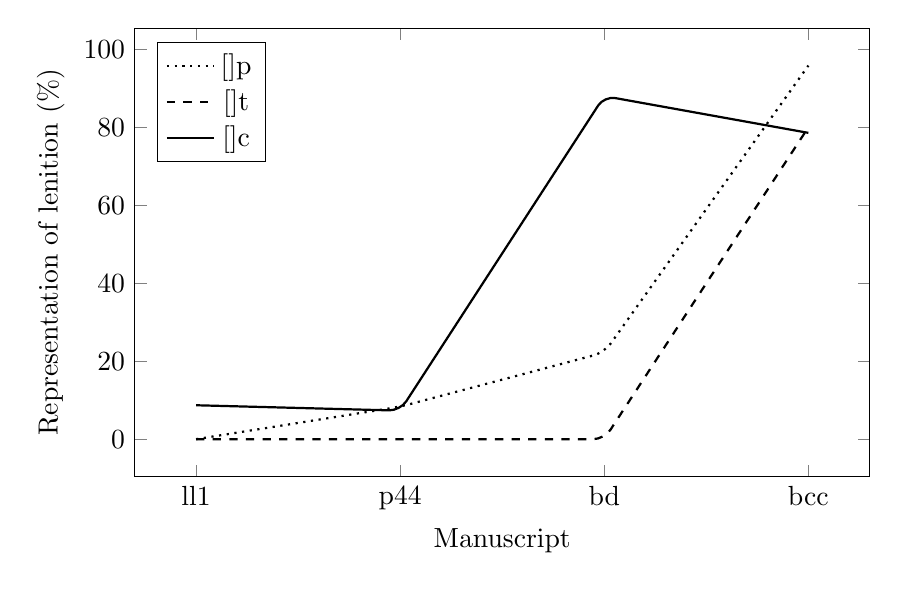
\begin{tikzpicture}
    \begin{axis}[
      width=.9\linewidth,
      height=.6\linewidth,
      xlabel=Manuscript,
      ylabel={Representation of lenition (\%)},
      symbolic x coords={
        \gls{ll1},
        \gls{p44},
        \gls{bd},
        \gls{bcc}
      },
      xtick=data,
      legend style={legend pos=north west},
      ]
      \addplot[color=black,rounded corners,thick,dotted,] coordinates {
        (\gls{ll1},0.00)
        (\gls{p44},8.33)
        (\gls{bd},22.22)
        (\gls{bcc},95.83)
      };
      \addplot[color=black,rounded corners,thick,dashed,] coordinates {
        (\gls{ll1},0.00)
        (\gls{p44},0.00)
        (\gls{bd},0.00)
        (\gls{bcc},80.00)
      };
      \addplot[color=black,rounded corners,thick] coordinates {
        (\gls{ll1},8.70)
        (\gls{p44},7.32)
        (\gls{bd},88.00)
        (\gls{bcc},78.57)
      };
      \legend{\mw[]{p},\mw[]{t},\mw[]{c}}
    \end{axis}
  \end{tikzpicture}
  \caption{Orthographical representation of voiceless stops over time.}
  \label{fig:linechartbrut}
\end{figure}

\subsection{Lenition in \acrshort{ll1} and \acrshort{p44}}
\label{sec:lenit-acrsh-acrsh}


The rule is clear in \gls{ll1} and \gls{p44}: lenition of voiceless stops is not written.
Given this rule, exceptions, constituting instances of representation of lenited voiceless stops, need to be accounted for.
These exceptions are found in Table~\ref{tab:ltrepll1p44}.
As can be seen in this table, both the form and meaning of the words themselves and their reason for being lenited differs, so accounting for them must be done on a case-by-case basis, and a satisfying account may not always be found.

\begin{table}[h]
  \centering
  \begin{tabular}{lddwql}
    \toprule
    \tch{Source} & \tch{Page} & \tch{Line} & \tch{Word} & \tch{Translation} & \tch{Reason lenition} \\
    \midrule
    \acrshort{ll1} & 34 & 1 & gellweyr & jest & \mw{trwy} \\
    \acrshort{ll1} & 35 & 8 & gytdỽundep & agreement & \mw{o} \\
    \acrshort{ll1} & 36 & 4 & gof & memory & \mw{ar} \\
    \acrshort{ll1} & 37 & 17 & glaf & sick & \mw{en} \\
    \acrshort{p44} & 25 & 10 & gewylyd & shame & \mw{en} \\
    \acrshort{p44} & 26 & 2 & gynt & before & adv phrase \\
    \acrshort{p44} & 26 & 9 & bryt & moment & \mw{pa} \\
    \acrshort{p44} & 27 & 6 & glaf & sick & \mw{en} \\
    \bottomrule
  \end{tabular}%
  \caption{Instances of \lT\ represented in \acrshort{ll1} and \acrshort{p44}.}
  \label{tab:ltrepll1p44}
\end{table}

One word that may be accounted for, however, is \mw[before]{gynt} (\gls{p44} 26.2).
It stands out in that it is the only lenited adverbial phrase in this source.
Moreover, lenition of adverbial phrases of time is often petrified, \eg \gmow[yesterday]{ddoe}.
The writing of \mw{gynt} with \mw{g} may similarly point to \gls{petr}, rather than \gls{morphophonlen}.
If so, this word constitutes a research exception.

The case of \mw[what moment?]{pa bryt} may be explained in a similar manner.
Although lenition following \mw{pa} is morphophonemic and still grammatical, it occurs frequently in combination with \mw{bryt}, so orthographical lenition is reminiscent of the \gls{petr} we find in research exception \mw[together]{y gyt}.
Comparison with phrases  such as \gmob[when]{peur < pe eur} also shows that interrogative pronouns containing \mw{pa} may be considered single words for the purpose of lenition.
Also, the semantics of the phrase obviously have a temporal dimension similar to \mw{gynt}.
The phrase \mw{pa bryt} is also found with exceptional lenition in \gls{bd}, as can be seen in Table~\ref{tab:replenpbd}.

After accounting for these two examples, we are still left with six examples of orthographically represented \gls{morphophonlen}.
These examples are few and far between, but nevertheless essential, because they show that lenition of voiceless stops \emph{could} be represented.
This means that writing \graph{b, d, g} for \lT\ had already been invented by the mid-thirteenth century.
It had just not been adopted widely.


\subsection{Lenition in \acrshort{bd} }
\label{sec:lenition-acrshortbd-}
In \gls{bd}, the rule is that lenition is not represented for \mw{p, t}, and it is represented for \mw{c}.
This rule is exceptionless for \mw{t}, but not for \mw{p} and \mw{c}.
These exceptions constitute instances where lenition is represented for \mw{p}, and for \mw{c} these exceptions constitute instances where lenition is not represented.
Table~\ref{tab:replenpbd} shows the two instances of orthographically represented lenited \mw{p}, and Table~\ref{tab:nonlencbd} shows every instance where lenited \mw{c} is not orthographically represented.

\begin{table}[h]
  \centering
  \begin{tabular}{addwql}
    \toprule
    \tch{Source} & \tch{Page} & \tch{Line} & \tch{Word} & \tch{Translation} & \tch{Reason lenition} \\
    \midrule
    bd & 34 & 4 & bryt & moment & \mw{pa} \\
    bd & 36 & 2 & baraỽt & ready & \mw{yn} \\
    \bottomrule
  \end{tabular}
  \caption{Representation of lenited \mw{p} in \acrshort{bd}}
  \label{tab:replenpbd}
\end{table}

\begin{table}[h]
  \centering
  \begin{tabular}{addwql}
    \toprule
    \tch{Source} & \tch{Page} & \tch{Line} & \tch{Word} & \tch{Translation} & \tch{Reason lenition} \\
    \midrule
    bd & 29 & 10 & caerussalem & (place name) & fem noun \\
    bd & 30 & 14 & kyuoeth & kingdom & \mw{y} ‘his' \\
    bd & 31 & 8 & kyuoeth & kingdom & \mw{y} ‘his' \\
    bd & 31 & 9 & kyuoeth & kingdom & \mw{y} ‘his' \\
    bd & 33 & 2 & caffei & received & \mw{na} \\
    bd & 35 & 1 & keissyaỽ & seek & \mw{y} ‘to' \\
    \bottomrule
  \end{tabular}%
  \caption{Non-representation of lenited \mw{c} in \acrshort{bd}}
  \label{tab:nonlencbd}
\end{table}

\subsection{Lenition in \acrshort{bcc}}
\label{sec:lenition-acrshortbcc}


Lenition of voiceless stops is as a rule represented in \gls{bcc}, so instances where lenition is not shown are the ones that need to be accounted for.
Table~\ref{tab:ltnotrepbcc} shows these instances of non-represented lenition.
Various reasons for lenition appear multiple times in this table.



\begin{table}[h]
  \centering
  \begin{tabular}{lddwql}
    \toprule
    \tch{Source} & \tch{Page} & \tch{Line} & \tch{Word} & \tch{Translation} & \tch{Reason lenition} \\
    \midrule
    \gls{bcc} & 16r & 29 & prosessio & procession & \mw{y} ‘to' \\
    \gls{bcc} & 16v & 6 & keluydodeu & arts & prep adj \\
    \gls{bcc} & 17r & 14 & kereis & I loved & \mw{th} \\
    \gls{bcc} & 17r & 15 & caraf & I love & \mw{th} \\
    \gls{bcc} & 17r & 16 & kerir & is loved & \mw{th} \\
    \gls{bcc} & 17v & 18 & tywyssauc & prince & apposition \\
    \gls{bcc} & 17v & 29 & tywyssawc & prince & apposition \\
    \gls{bcc} & 18r & 12 & trugarhae & mercy & \mw{y} ‘his' \\
    \gls{bcc} & 18r & 25 & Cordeilla & (personal name) & \mw{-ei} \\
    \gls{bcc} & 19r & 10 & Cordeilla & (personal name) & \mw{-ei} \\
    \gls{bcc} & 19v & 4 & tywyssawc & prince & apposition \\
    \gls{bcc} & 19v & 4 & tywyssawc & prince & apposition \\
    \gls{bcc} & 19v & 5 & calet & hard & prep adj \\
    \gls{bcc} & 19v & 13 & cordeilla & (personal name) & \mw{y} ‘to' \\
    \gls{bcc} & 19v & 25 & creftwyr & craftsmen & prep adj \\
    \bottomrule
  \end{tabular}%
  \caption{Instances of \lT\ not represented in \acrshort{bcc}.}
  \label{tab:ltnotrepbcc}
\end{table}

Within \gls{bcc}, \mw[prince]{tywyssawc} is found four times in apposition to a personal name.
A lenitable noun in apposition to a personal name is found eight times within this source, and is lenited only once in \mw[prophet]{broffwid} (\gls{bcc} 16r.26).
Lenition of nouns in apposition is not shown for other types of consonants either, as the word \mw[king]{brenhin} is also found in unlenited form in this position.

The word \mw{prosessio} is a late, learned loanword from \glat[procession]{prōcessiō}.
Writing \glat{c} in this word with \mw{s} confirms a post-vernacular pronunciation.
Phonologically, the structure of the word does not look Middle Welsh, as /au/ had not yet turned into /o/ in the final syllable.
This means that \mw{prosessio} constitutes an instance of code switching, or a recent loan.
Recent and transparent loanwords are not typically mutated in \gls{mow}, nor are instances of code switching.

The personal name \mw{Cordeilla} is found unlenited where lenition is expected on three separate occasions.
The fact that we are dealing with a personal name here may be of influence, as \mw{llyr} is found unlenited following \mw[fort]{caer} twice.
Furthermore, personal names are as a rule not lenited in \gls{mow}.
These instances of \mw{llyr} and \mw{Cordeilla} may be early examples of this \gls{mow} rule.
Additionally, \mw{Cordeilla} is a foreign name for the Welsh, and it may thus not have been lenited similarly to \mw{prosessio}.

Infixed object pronoun \mw{'th} should cause lenition, but this is not found in \gls{bcc}.
Lenition is problematic diachronically, as this pronoun causes provection in \gls{mco} and \gls{mb}.
Arguably, provection following this pronoun is also found in \gow[as it brings you]{imalitiduch} where medial \ow{t} represents both the /θ/ of the object pronoun, and preverb \ow{di} > \ow{ti}.

Several words following a preposed adjective fail to show lenition, although these instances are outnumbered by preposed adjectives shown to cause lenition.
Lenition following preposed adjectives is a type of free lenition, because all adjectives cause lenition when used as a preposed adjective.
These same adjectives do not as a rule cause lenition when they are in their usual postnominal position.
Consequently, the correct application of lenition hinges on the morphosyntactic relationship between two elements in the same clause rather than by simply checking whether the immediately preceding morpheme should cause lenition.
This morphosyntactic relationship may not always be clear or consistent.
Preposed adjectives are more frequent in this text than in \gls{mw} in general, because it is a translation from Latin, which further increases the likelihood of inconsistencies in the application of preposed adjectives.
An example where lenition following a  preposed adjective is to be expected is Example~\ref{ex:wychyrcalet}:
\mwcc[ex:wychyrcalet]{\gls{bcc} 19v.3--6}{ac yn ev herbyn wynt y doeth Maglawn tywyssawc yr alban. a henwyn tywyssawc kernyw ac ev holl allu. ac ymlad yn \al{wychyr calet} ac wynt.}{And against them came Maglawn, prince of Scotland, and Henwyn, prince of Cornwall, and their whole capability, and they fought \al{violently hard} against them.}
What exactly is the grammatical relationship between \mw[violent]{wychyr} and \mw[hard]{caled}?
Is \mw{wychyr} a preposed adjective followed by lenition, and translating to the translation given, or does \mw{caled} modify \mw{wychyr}, and are we not to expect lenition here?
In the latter case, `very violently' would be a more suitable translation%
\footnote{The Latin original is of little help either, as it is much terser than the Welsh: \lat[When this was done, Leir took his daughter and the assembled army to Britain. He fought with his sons-in-law and beat them.]{Quo facto, duxit secum leir filiam et collectam multitudinem in Britanniam pugnauitque cum generis et triumpho potitus est.}~\autocite[42--43]{Geo_History09}}.
And does the meaning matter at all for lenition?
At any rate, non-lenition is consistent, as the \mw{Brut} found in \gls{bcc} has four different instances of \mw{wychyr calet}, and each of them keeps the radical: 19v.5, 25v.14, 47v.12, 51r.29.
\Textcite[31--32]{morgan_y_1952} argues that constructions of the type  \mw{yn} + adjective + adjective  may be considered dvandva compounds or as compounds where one adjective typically has an intensifying function.
In any case, the repetition of adjectives constitutes the creation of a compound adjective, and thus always cause lenition, but that southern dialects tend to keep the radical here.
If Morgan is right, the example of  \mw{wychyr calet} seems like an aberration in both cases, because the second element should be lenited irrespectively of its semantics.
In the end, non-lenition may be a purely southern dialectal feature.

Many exceptions to the representation of lenition in \gls{bcc} stem from the difficulties involved in translating a Latin text.
After accounting for these, lenition seems to have been applied with great regularity, and remaining exceptions seem no more numerous than what is found in a \gls{mow} text of similar length, barring only the most carefully copy-edited ones.
As such, \gls{bcc} demonstrates that lenition of voiceless stops was wholly represented by the mid-fourteenth century.

\section{Lenited \mw{g}}
\label{sec:lenited-mwg}
The only number in Table~\ref{tab:perlenbrut} or Table~\ref{tab:perlenbrutex} not referring to a voiceless stop and dipping below the fifty per cent mark is that of the representation of lenited \mw{g} in \gls{p44}.
This begs the question why \mw{g} in \gls{p44} --- and to a lesser
extent in \gls{ll1} --- is lenited so infrequently.  In \gls{ll1}
lenited \mw{g} is shown in 49 out of 68 instances; in \gls{p44} it
is written in  only 26 out of 72 instances.  The element causing lenition
does not seem to be relevant, \eg verbal particle \mw{a} regularly
causes lenition to \mw[did]{oruc}, but not to \mw[did]{gwnaeth}.

The phonology of the lenited word does seem to play a role: when
initial \mw{g} is not followed by \mw{w}, it disappears in 48 out of
52 of such instances. The remaining four comprise the following
instances: \mw[they rested]{gorffowyssassant} (\gls{ll1} 38.25),
\mw[rested]{gor/ffowyssỽs} (\gls{p44} 23.9--10), \mw[gain]{gorescyn}
(\gls{p44} 27.15), and \mw[glorious]{gogonedỽs} (\gls{p44}
28.23). These words all historically started with \mw{g\cw}, but  \mw{\cw}
preceding \mw{o} has disappeared by the end of the \gls{ow} period. However, such words
starting with \mw{go} do represent lenition elsewhere, such as in the
plentiful instances of \mw[did]{oruc}.

The remaining 88 instances are all words starting with \mw{(g)w}, of which 27 show lenition.
Table~\ref{tab:gwphon} shows that the phonological structure of these words plays an important role in dictating whether lenition is written.
If the \mw{w} following lenited \mw{g} is vocalic, lenition is usually shown.
An example of such a word showing lenition is \mw[husband]{wr} (\gls{ll1} 34.13).
Similarly, lenition is usually shown if the quality of the following \mw{\cw} is consonantal, if this consonant is in turn followed by a vowel, \eg \mw[wear]{wyscaỽ} (\gls{p44} 27.7).
However, if the \mw{g} is followed by consonantal \mw{\cw}, and then followed by yet another consonant, lenition is usually not written, \eg \mw[make]{gwneỽthỽr} (\gls{p44} 27.28).

\begin{table}[h]
  \centering
  \begin{tabular}{ldd}
    \toprule
    & \tch{\graph{w}} & \tch{\graph{gw}}\\
    \midrule
    /ɡ\cw{}\gls{C}/ & 3 & 48\\
    /ɡ\cw{}\gls{V}/ or /ɡu/ &24 &13\\
    \bottomrule
  \end{tabular}
  \caption{Lenition of \mw{gw} divided by phonological structure of the word.}
  \label{tab:gwphon}
\end{table}

Not representing lenited \mw{g} served a purpose: it served to distinguish consonantal \mw{w} from its syllabic counterpart if it followed \mw{g} and preceded a consonant.
Maintaining  radical \mw{g} in the face of lenition served to indicate that the following \mw{\cw} before another consonant was consonantal, so that no reader of a phrase like \mw[his wife]{ẏ gwreic} would ever be fooled into saying /i ur\dots/ before reading the rest of the phrase and having to correct himself to /i \cw raɪɡ/.

\section{Conclusion}
\label{sec:conclusion-brut}
Lenition of voiceless stops was generally not written in the early thirteenth century, but it was not unfamiliarity with the concept of using \graph{b, d, g} for historical \mw{p, t, c} that kept them from writing lenition as such.
After all, these letters were used for \gls{petr}, and in exceptional cases even for \gls{morphophonlen}.
In the late thirteenth century, lenited \mw{c} came to be written as \mw{g}, but a similar shift did not occur for \mw{p} and \mw{t}.
These  departures from the thirteenth-century norm give us one key insight: lenition could be represented by this period, it had just not become the norm yet.

The case of lenited \mw{g} shows how the question of whether and how to write lenition may interplay with seemingly unrelated conundrums. 
A scribe who wished to ensure that no consonantal \mw{\cw} was mistaken for a vocalic \mw{w} had to weigh this wish against his wish to write lenition.
The former wish took precedence for the scribes of \gls{ll1} and \gls{p44}, and their priorities make sense in an orthographical tradition where the writing of lenition was limited to only several consonants, and where ability to read out loud would have been held in high esteem.

So what was the conundrum for voiceless stops?
What wish had to be weighed against the wish to represent lenition of these consonants?
The obvious answer to this question is that \lT≠\xD.
If lenited voiceless stops had not yet merged with radical voiced stops word-initially, then confusing the two when speaking might have been just as embarassing as using a vocalic \mw{w} for a consonantal \mw{\cw}. 
According to this line of reasoning, the phonological distinction between \lT\ and \xD\ argued for in Part~\ref{part:phonology-phonetics} must have survived until the middle of the thirteenth century.

\todo[inline,caption={gg}]{For General conclusion: this means that not showing \lT\ is evidence of a early composition; probably dating back to  the period when they had not yet merged with \xD. However, the \mw{Brut} also shows that not writing \xD\ = \lT\ was by {choice}, rather than {ability}. They were able to write \lT\ like \xD\ as early as the thirteenth century, but they had to weigh representation of lenition against  the correct pronunciation of \lT\ separate from \xD. Another scribe (\eg of the Book of Aneirin) may have had different priorities, and could represent lenition of \lT. Ergo, writing lenition of \lT\ is not by itself a marker of lateness, but not writing lenition of \lT\ is, by contrast, a marker of earliness.}
%%% Local Variables:
%%% coding: utf-8
%%% mode: latex
%%% TeX-master: "../main"
%%% End:
